% \subsection{Introduction and Motiv<ating Example}
% \label{subsec:carol-example-introduction}


EpiMDE is designed to support workflow extensions implemented as separate layers on top of the core platform. It exposes the metamodel and model repository through an EMF based API, enabling external analyses (e.g., clustering, differencing, logical consistency checks) to be integrated without modifying the platform itself. In our third case study, we examine how well EpiMDE supports epidemiological workflows, by developing an illustrative example. 
Specifically, we use a rapid prototyping scenario~\cite{fiyouzisabah2024towards} to probe whether the platform provides sufficient expressiveness and extensibility to support the construction of workflow-specific tooling on top of EpiMDE.
% Specifically, we probed how well the platform can be used to build a tool for rapid prototyping of epidemiological models, in a context that arises when a new disease is discovered. 
We studied the research question: 
\textit{What challenges and opportunities arise when applying a purpose-built modeling infrastructure to the development of domain-specific modeling workflows?} 
The lessons learned reveal both the platform’s strengths and its friction points.

We assume a persona named ``Carol'' working under the pressure of a health crisis (like the COVID-19 pandemic) to quickly create and validate an epidemiological model. 
Carol hopes to rapidly prototype a new model by reusing previously developed, tested, and validated model components to accelerate her work. 
So, she wants to identify and select useful modeling elements and assemble them into a partially completed prototype, avoiding redundant re‐implementation efforts. 
She hopes that, using this prototype model as a base, she can focus on her study's unique aspects and design and integrate new features. 
All models and generated artifacts from our scenario are included in our replication package published on Zenodo~\cite{zenodo_17806440}.

We assume that Carol starts with a corpus made up of the three previously developed compartmental models shown in Figure~\ref{fig:prototype_submodels}. 
Each one contains elements that may be relevant and useful for her own study. 
For instance, the model $m_1$ in Figure~\ref{fig:prototype_m1} includes exposed and vaccinated groups.
The model $m_2$ in Figure~\ref{fig:prototype_m2} adds more details about disease spread by breaking down the infectious population into asymptomatic, mildly symptomatic, and severely symptomatic compartments. 
Finally, the model $m_3$ in Figure~\ref{fig:prototype_m3} contains the hospitalization status of individuals, allowing to better model the load to the healthcare system.
Typically, Carol would have to manually search through the corpus of existing models, identify which parts are relevant, extract them, and then integrate them into her own model.
This is time-consuming and error-prone. 
Using the EpiMDE platform, we can simplify this process by creating an interactive layer that guides users like Carol through the steps for reusing previous work. 
Carol only needs to provide a repository of existing models. 
The tool then follows the workflow explained later (see Subsection~\ref{sec:prototyping_workflow}) to analyze these models and identify potentially relevant components. 
Finally, Carol can select the parts she wants to reuse, and the tool will automatically generate a prototype model that includes the selected items. 
She can then use this as a partially completed prototype on which to base the rest of her modeling efforts. 

\begin{figure}[t]
\centering
\begin{subfigure}[b]{0.40\textwidth}
  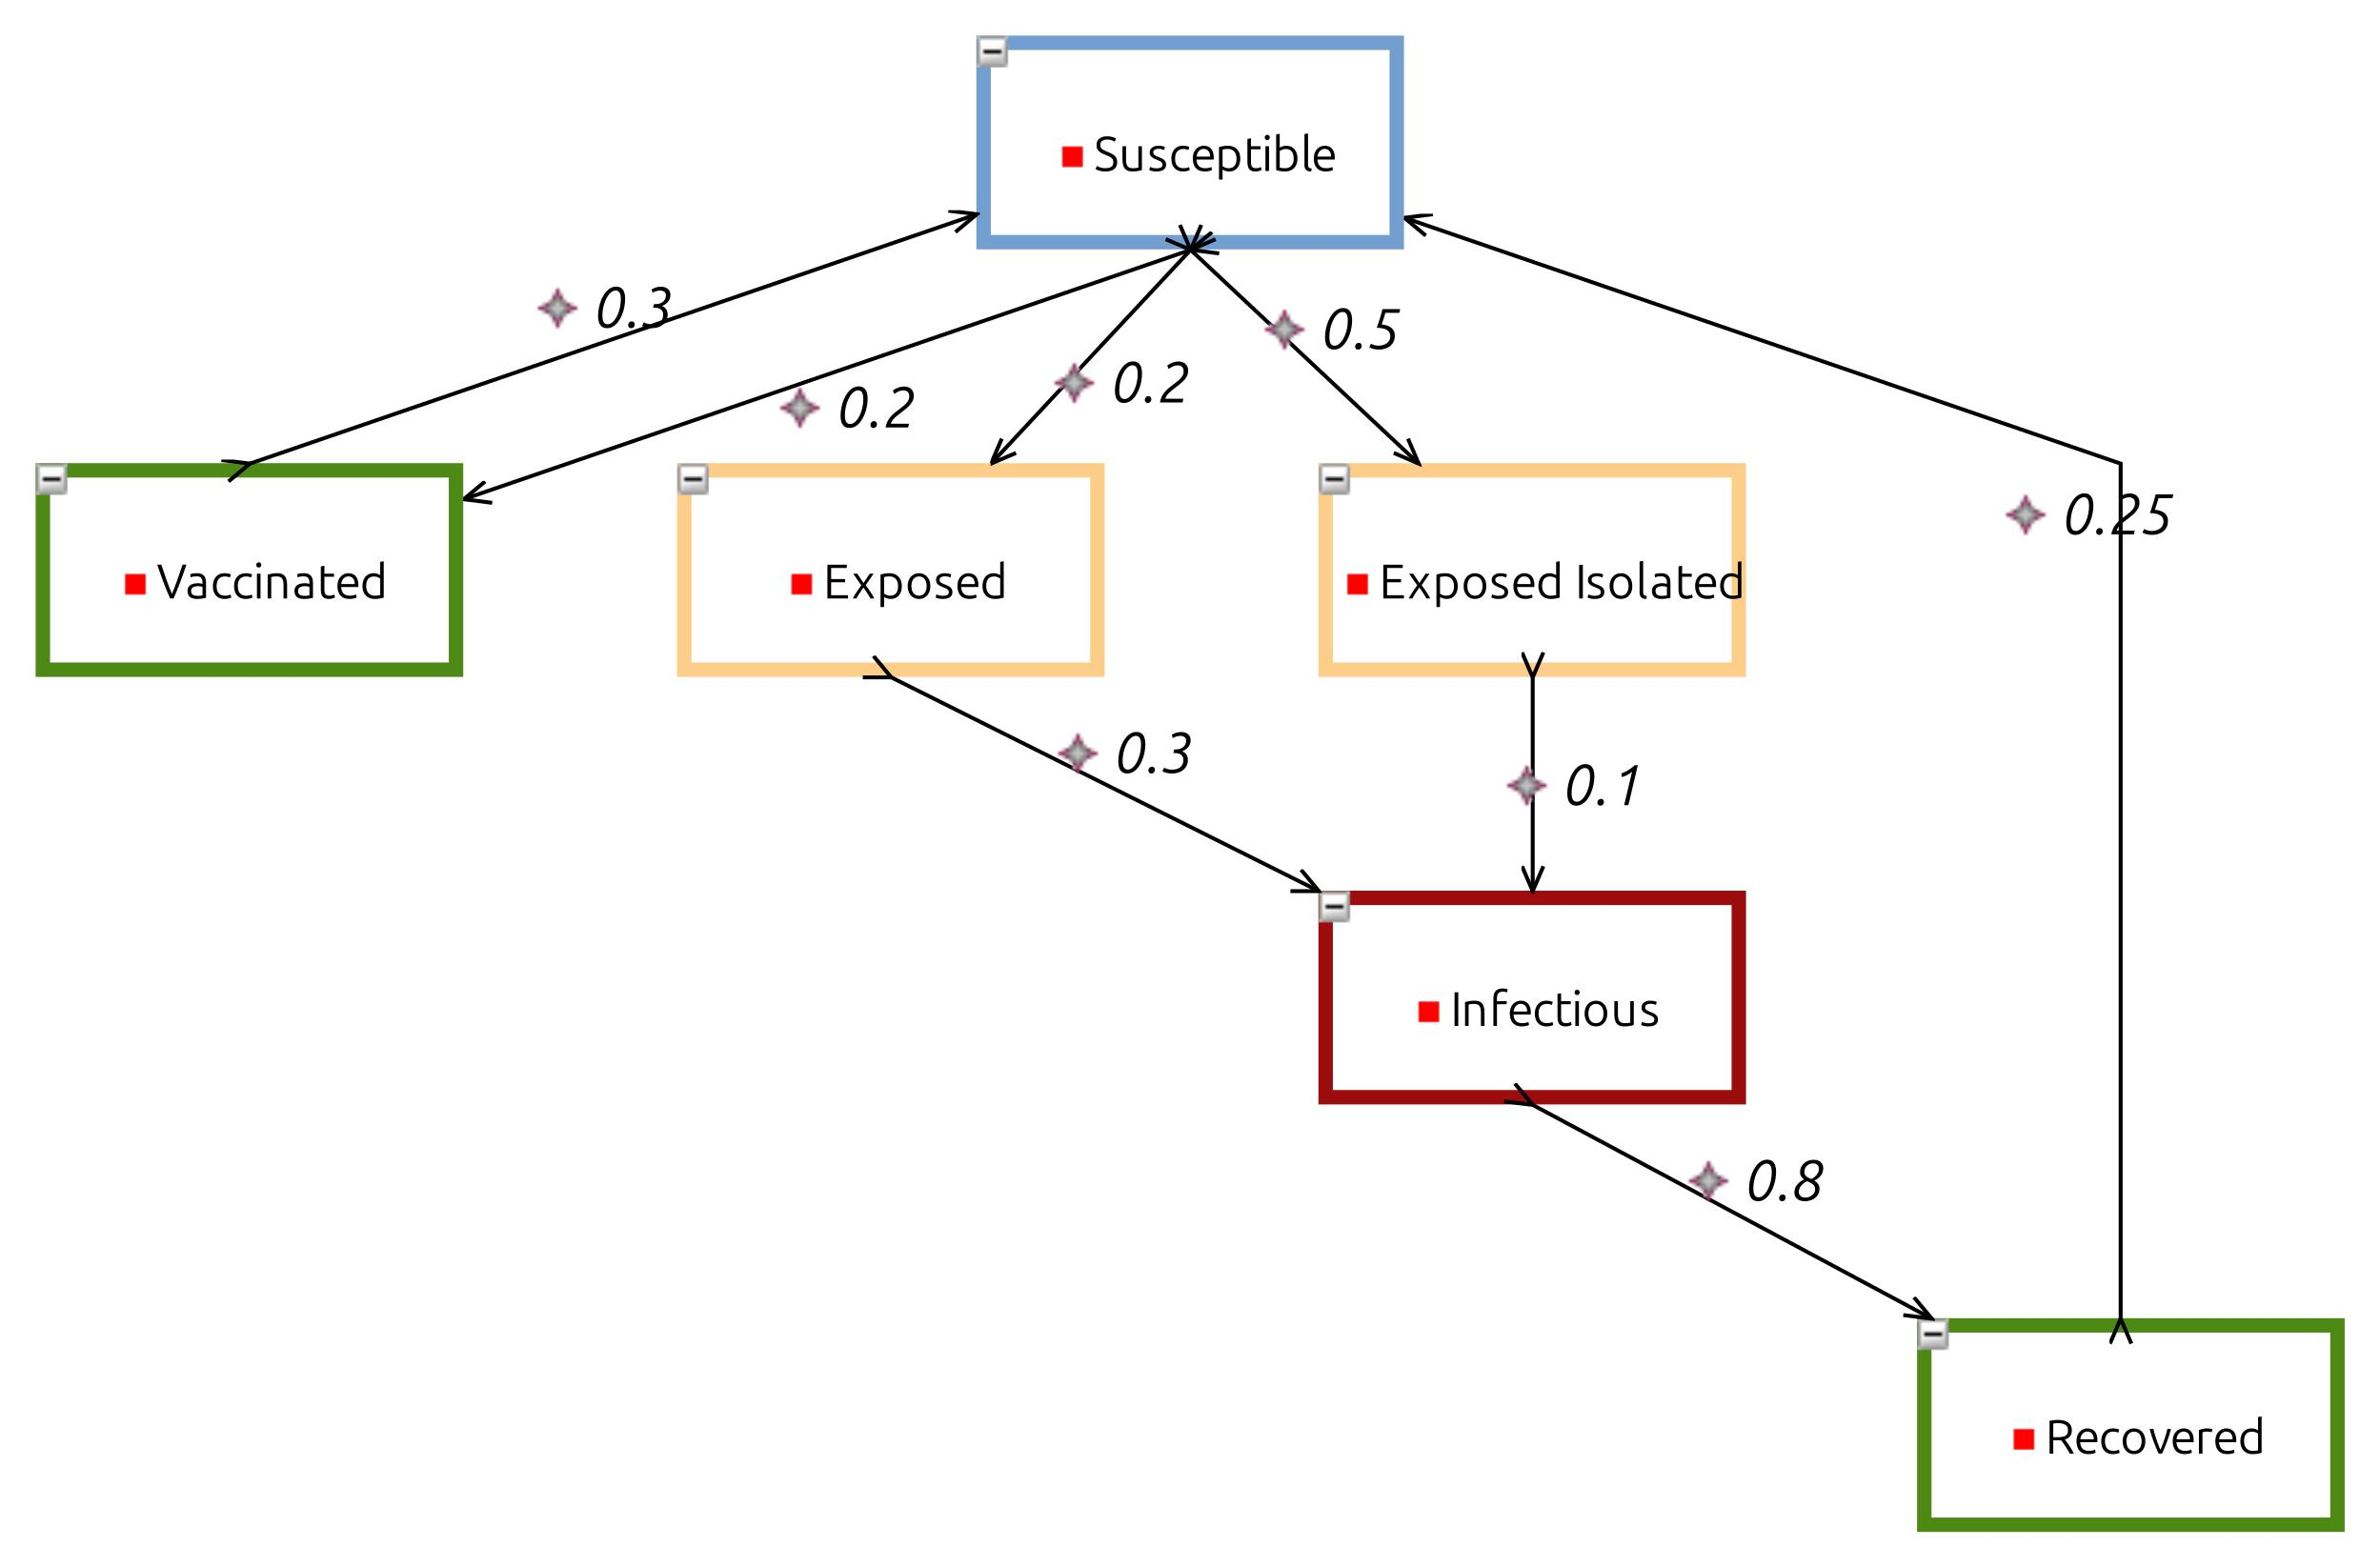
\includegraphics[width=\textwidth]{Figures/paper1.jpg}
  \caption{$m_1$}
  \label{fig:prototype_m1}
\end{subfigure}
\begin{subfigure}[b]{0.40\textwidth}
  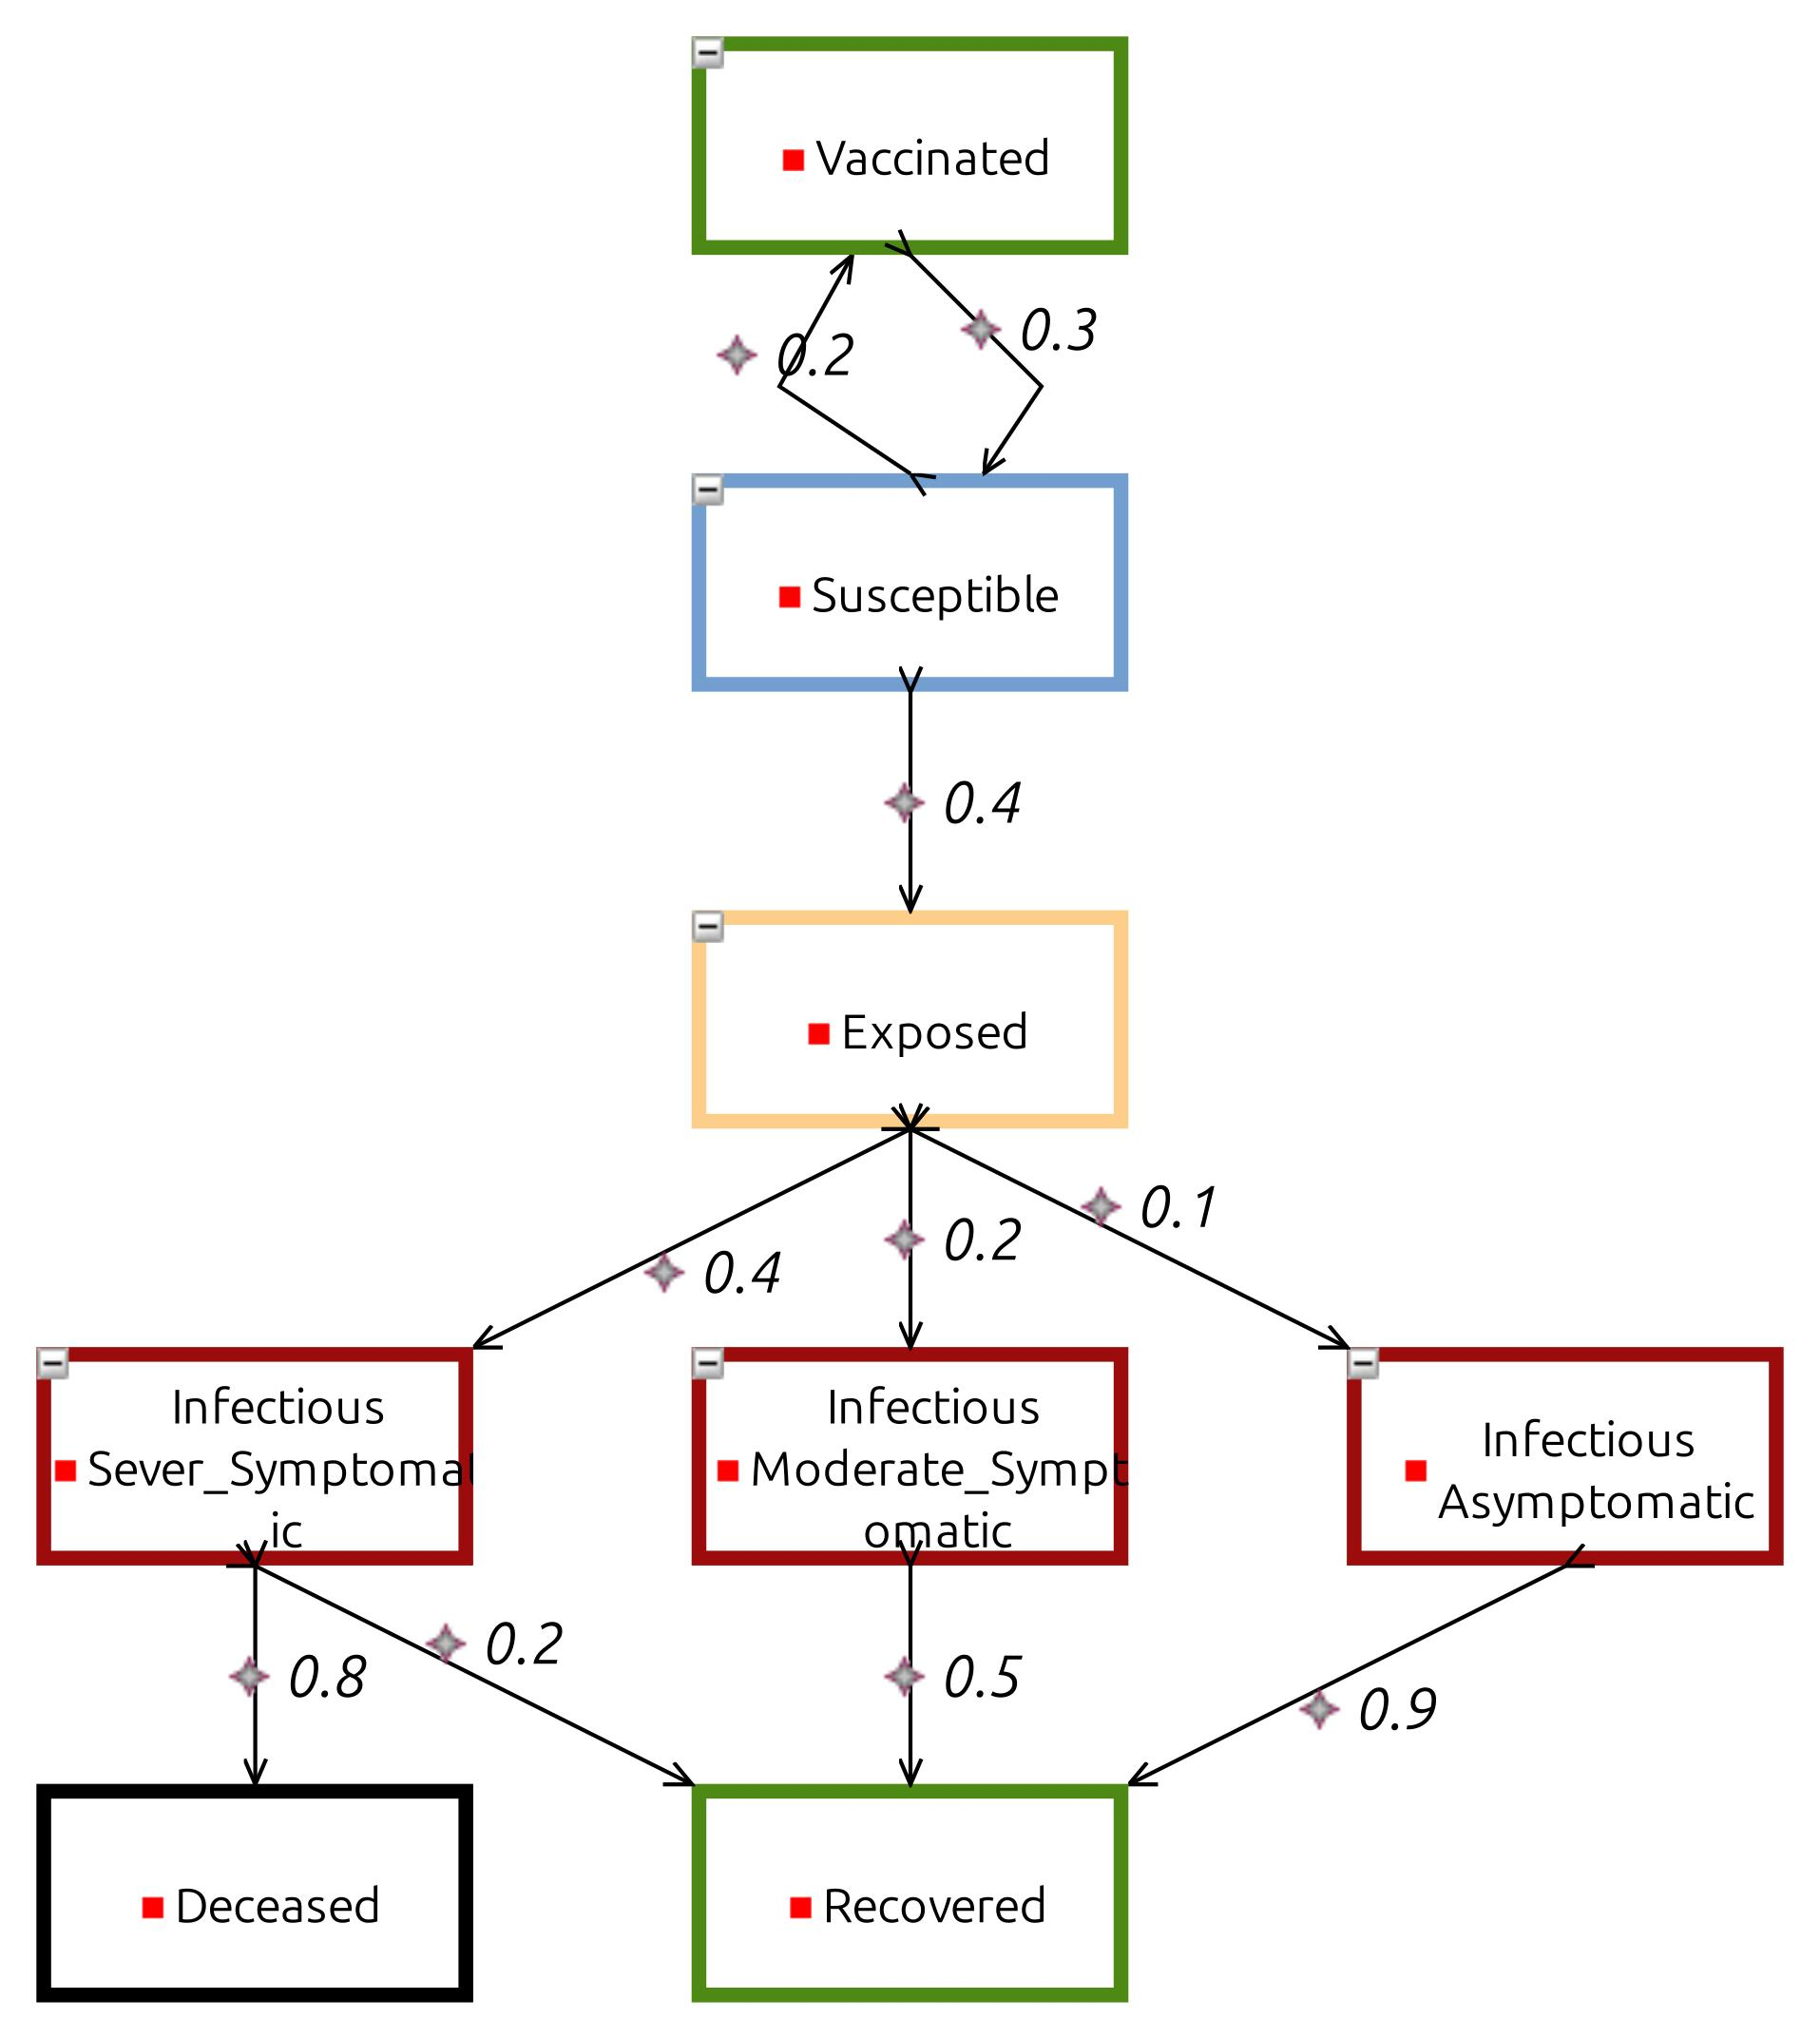
\includegraphics[width=\textwidth]{Figures/paper2.jpg}
  \caption{$m_2$}
  \label{fig:prototype_m2}
\end{subfigure}
\begin{subfigure}[b]{0.40\textwidth}
  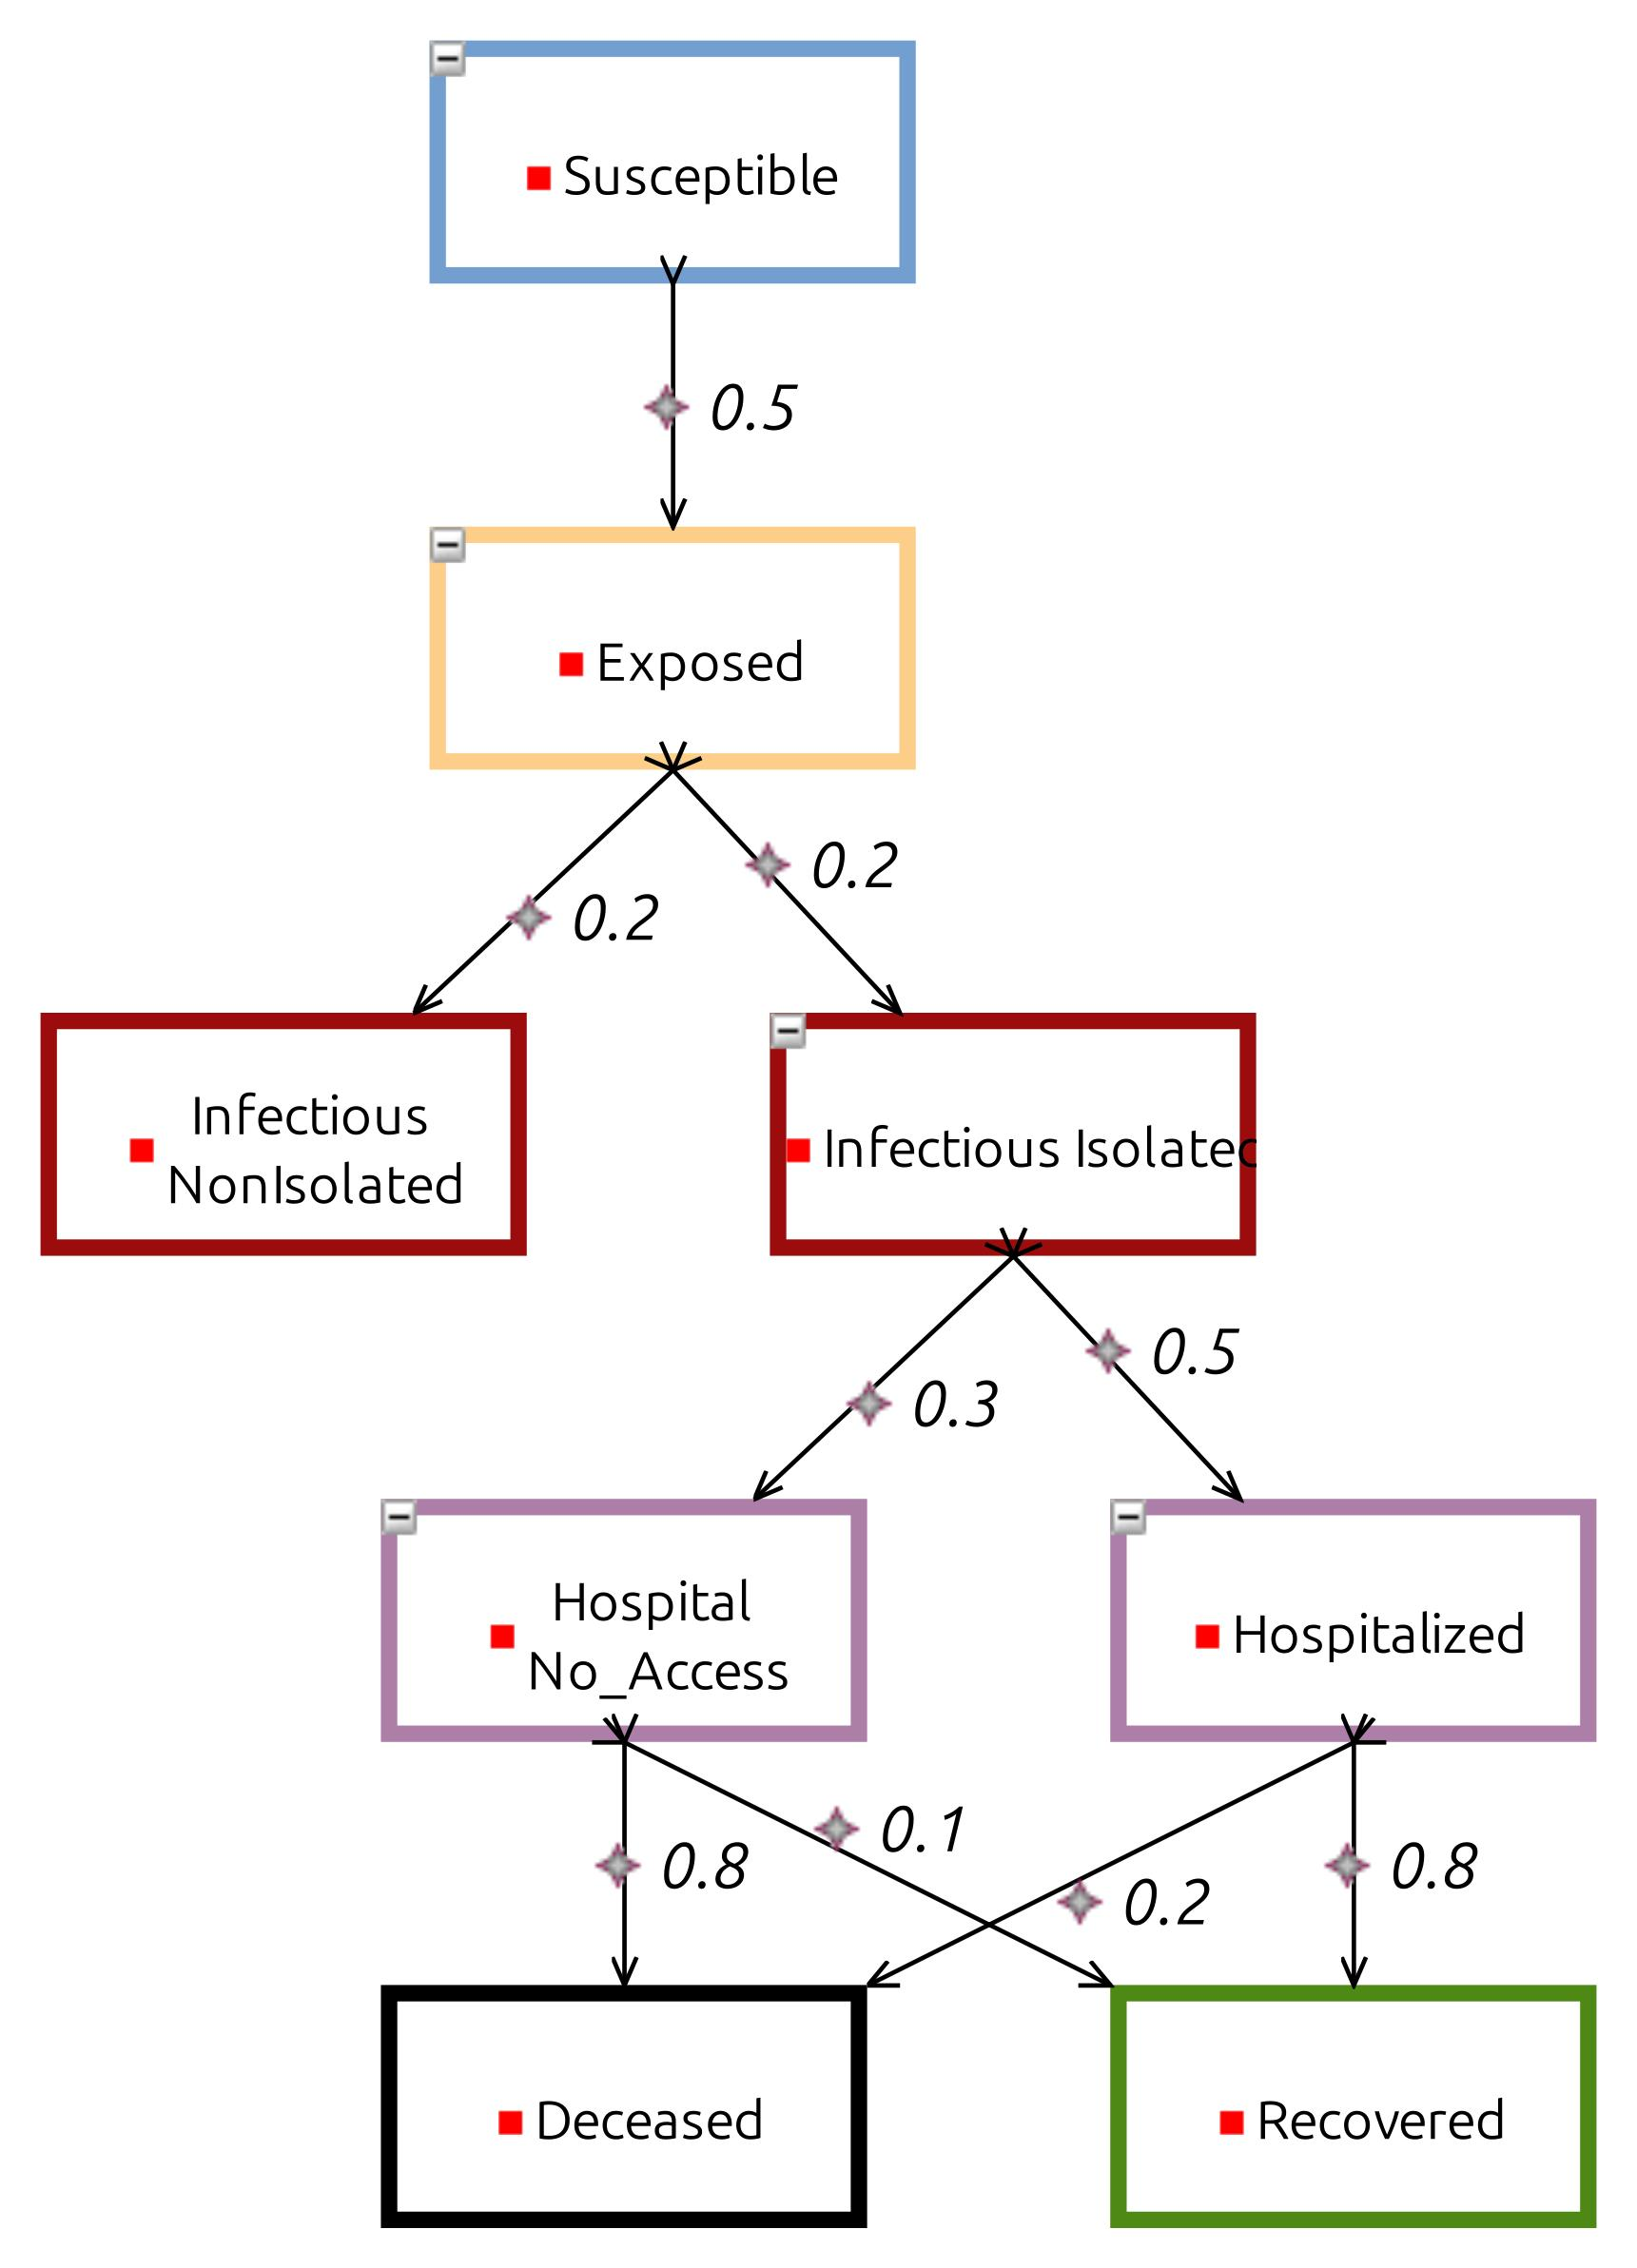
\includegraphics[width=\textwidth]{Figures/paper3.jpg}
  \caption{$m_3$}
  \label{fig:prototype_m3}
\end{subfigure}
\caption{Corpus of prior compartmental models to consult.
}
\label{fig:prototype_submodels}
\end{figure}

% \subsection{Approach}
%to help epidemiologists seamlessly reuse modeling ideas from previous models and rapidly integrate them into a prototype model, which they can use for further development. Below, we explain the four steps of our approach.

\subsubsection{Workflow}
\label{sec:prototyping_workflow}

We implemented the workflow as an external layer on top of EpiMDE. It operationalizes a prototyping-specific notion of ``relevance'' to support rapid model construction under time pressure. EpiMDE itself does not prescribe a canonical relevance metric or workflow; rather, it provides the model representations, APIs, and analysis hooks required to implement such workflows.

Concretely, the workflow layer leverages programmatic access to EpiMDE models and metamodel instances, stable element identifiers, and integration with third-party analysis tools. The heuristics used to identify and rank potentially relevant components are intentionally workflow-specific, and are presented here to demonstrate that EpiMDE provides sufficient expressive power and extensibility to support domain-specific modeling workflows.

We build the interactive rapid prototyping EpiMDE layer in four steps.

\paragraph{Variation Point Extraction:} 
First, we identify commonalities and differences in the input corpus.
For example, the compartment \textit{Susceptible} appears in all models ($m_1$-$m_3$), so we consider it a commonality indicating the same epidemiological concept. 
On the other hand, the compartment labeled \textit{Hospitalized} only appears in $m_3$: the other models do not concern themselves with this concept.

Note that although the models in the corpus may describe different diseases, identifying variation points remains meaningful. Many epidemiological concepts, such as the \textit{Susceptible} compartment, represent fundamental population states rather than disease-specific mechanisms. Thus, commonalities can still capture shared modeling structures that are valuable for constructing new prototypes even when the models target distinct pathogens. Of course, if the input corpus contains models of the same disease, the identified variation points are likely to be more disease-specific and semantically aligned.

To systematically identify \textit{variation points}, we assign unique identifiers (IDs) to the model elements, as follows: 
%A variation point represents a model element in a way that allows us to determine whether it is shared across models or distinct. The IDs are defined as follows:
%\begin{itemize}
    %\item 
(a) For compartments, the ID is simply the name of the compartment.
    %\item 
(b) For rates, flows, etc., the ID is a combination of the source compartment ID, target compartment ID, and the flow rate expression.
%\end{itemize}
%
When two elements share the same IDs, they are considered the same, but if their IDs are different, they are treated as variants. 
%This step helps identify common parts shared among models, laying the groundwork for extracting meaningful \textit{features} in the next steps.

% In the first step, our tool extracts the variation points from the existing models that Carol intends to reuse.
In Carol's case, for example
%an ID to each model element to identify which variation points are shared or unique across models. For compartments, we use the compartment name as the Variation Point ID. For example,
in model $m_1$, EpiMDE creates IDs for compartments such as \textit{Susceptible} and \textit{Vaccinated} %, and \textit{Exposed}.% are treated as distinct variation points. 
and IDs for flows such as %the ID is constructed by combining the source and target compartments as well as the flow rate. For instance, 
$Susceptible\_Vaccinated\_0.2$. 
%refers to a flow from \textit{Susceptible} to \textit{Vaccinated} with a rate of 0.2. 
% Using these IDs allows the tool to consistently detect and assign variation points to models. 
We show the complete list of variation points assigned to the models $m_1$, $m_2$, and $m_3$ in the Appendix Table~\ref{tab:prototype_variation_points}.


\paragraph{Feature Identification:} 
Next, we identify collections of variation points that appear together in the corpus and cluster them accordingly. 
These clusters likely represent features~\cite{berger2015feature}, pending confirmation by the epidemiologist.
We use Formal Concept Analysis (FCA), a mathematical framework used in data analysis and knowledge representation~\cite{ganter2012formal}
to classify objects based on shared attributes. 
Specifically, we integrated EpiMDE with FCA4J library~\cite{gutierrez2022fca4j}, 
which allows us to identify recurring patterns based on their shared variation points.%, identified by their unique IDs. 
%This allows us to detect shared variation points across different models, 
%that appear as recurring patterns that may represent modeling ideas or specific concepts that can be meaningfully reused together. 
%We then cluster these variation points to
We can thus identify potentially reusable components derived from existing models.
%
EpiMDE does this interactively, allowing Carol to change the automatically identified clusters.
This gives the epidemiologist the flexibility to split or reorganize clusters in case the mechanical clustering missed some relevant semantic nuance.
%This flexibility is important as some clusters might contain elements that are not related to each other, or the epidemiologist may prefer to reorganize them based on the specific needs of their study. 
We further prompt the epidemiologist to assign a meaningful label to each cluster. 
%These labels will make it easier for them to refer to and recognize the clusters further in the process. 
Once finalized and labeled, the refined clusters are henceforth referred to as \textit{features}. 


For Carol's three models
%In the second step, we apply Formal Concept Analysis (FCA) to the three models and their associated variation point IDs. 
FCA detects maximal groups of models that share a maximal set of variation points. 
We then cluster each of the identified sets of shared variation points to show the potential building blocks of existing models. 
For example, FCA identifies that all models share $Susceptible$, $Exposed$, and $Recovered$, which we put in the same cluster. 
% This set is identified by FCA, and we put them into the same cluster. 
This suggests that they often appear together and may represent a commonly reused pattern. 
Another example is the cluster formed by $Vaccinated$, $Susceptible\_Vaccinated\_0.2$, and $Vaccinated\_Susceptible\_0.3$, shared between $m_1$ and $m_2$. 
The fact that these co-occur in more than one place, indicates they might represent a common modeling idea that Carol would want to reuse together.

As a result of this step, EpiMDE generates the Appendix Table~\ref{tab:prototype_clusters}, which presents the clustered variation points. 
The table also includes a \textit{ClusterLabel} column initially left blank, allowing Carol to assign meaningful labels to each cluster. 
Carol can also refine and adapt the clusters as needed. 
We assume that she assigns the labels shown in the \textit{ClusterLabel} column and leaves the automatically identified clusters unchanged. 
Based on Carol's decision, each row in Table~\ref{tab:prototype_clusters} is considered to contain one \textit{feature}. 



\paragraph{Feature Relationship Identification:} Next, we identify relationships between features, such as dependency or mutual exclusivity. 
We always identify two relationships by default: 
%\begin{itemize}
    %\item 
(a)    A feature that contains a flow is always dependent on any other feature(s) containing the flow's source and target compartments. This ensures that compartments are well formed graphs.
    %This ensures that if we want to include the former in the prototype model, we also include the latter.
    %\item 
(b)    We assume that only one flow can exist between two compartments\footnote{Since compartmental models visualize differential equations, multiple arrows between the same compartments are redundant: they can be collapsed into a single arrow labeled with the sum of the rates. For our purposes, where the goal is to identify variation points between models, we treat differing rates as mutually exclusive alternatives, rather than cumulative effects.}. Thus if a feature contains a flow between two Compartments $A$ and $B$, it is mutually exclusive to  features that include other flows between $A$ and $B$.
%\end{itemize}
EpiMDE also prompts the epidemiologist to refine, customize and extend the set of identified feature relationships.
The resulting set of relationships are encoded in propositional logic, using the LogicNG library~\cite{logicng}.

In Carol's case, 
%In the next step, considering the features and the variation points each one contains, we identify the logical dependencies between features.
EpiMDE by default identifies the relatioship $Vaccination \Rightarrow Core\_SER$. 
This is because the $Vaccination$ feature includes a flow from \textit{Susceptible} to \textit{Vaccinated}. 
This flow relies on the existence of the $Susceptible$ compartment, which is part of the $Core\_SER$ feature, so $Vaccination$ depends on $Core\_SER$. 

Carol's case also includes mutual exclusivity relationships between features, such as the relationship
$Symptom\_Severity \Rightarrow \neg{Isolated\_Hospital} \land \neg{Exposed\_Isolation\_States}$. 
This is because $Symptom\_Severity$ has a flow from \textit{Susceptible} to \textit{Exposed} with a rate of 0.4, 
while $Isolated\_Hospital$ and $Exposed\_Isolation\_States$ also have flows between the same two compartments but with different rates. 
Based on our assumption that a compartmental model does not contain multiple flows between the same source and target compartments, 
EpiMDE identifies these features as mutually exclusive. 
The full set of the identified logical dependencies between features in Carol's example is available in the Zenodo replication package~\cite{zenodo_17806440}. 
In EpiMDE, Carol can further review, edit, or add to these constraints as needed. 




\paragraph{Feature Selection and Prototype Generation:} %With the features and necessary logical relationships between them at hand, it is time to construct the prototype model. 
To construct the prototype, Carol is prompted to select which combination of features she wants to include in her prototype.
%We ask the epidemiologist to select the features to include in their prototype model. 
%Providing a labeled list of features, using the labels that the epidemiologist assigned, makes it much easier for them to recognize and choose the relevant features that they want to include based on their specific modeling goals.
The epidemiologist can do this using the feature labels defined in Step 2.
%
To ensure her selection is valid with respect to the dependencies identified in Step 3, 
EpiMDE conjuncts all relevant relationship formulas and makes a satisfiability check using LogicNG. 
%the validity of user selection, we check its satisfiability according to the defined dependency rules, using an SAT solver along with the previously constructed LogicNG logical formulas. 
If the result is UNSAT, the epidemiologist is given a warning and asked to adapt her feature selection.
%If the solver finds the selection unsatisfiable, it means the combination of selected features does not work together logically. 
With a valid feature selection, we generate a prototype compartmental model that includes the appropriate features.
We implemented the feature merging in Java using the EpiMDE metamodel.

In Carol's case, EpiMDE prompts her to select from the list of features to include in the prototype model. 
We suppose that she selects $Mortality$ and $Exposed\_Isolation\_States$. 
EpiMDE checks for the satisfiability of the logical dependencies of her selection. 
They are satisfiable, and EpiMDE generates the model shown in Figure~\ref{fig:prototype_result_model}. 
In addition to Carol's selected features, the prototype model contains the feature $Core\_SER$, which Carol did not directly choose, but it is required based on the logical relationships between features. 
Carol can then treat this generated model as a prototype that reuses features from previous models.
She can then use it as the basis to develop a complete model according to her needs, without having to re-implement these features.
%completed, meaning that while it contains the desired features from existing work, Carol can evolve it further and add novel aspects specific to her study. 

% \end{enumerate}

 
\begin{figure}[t]
  \centering
  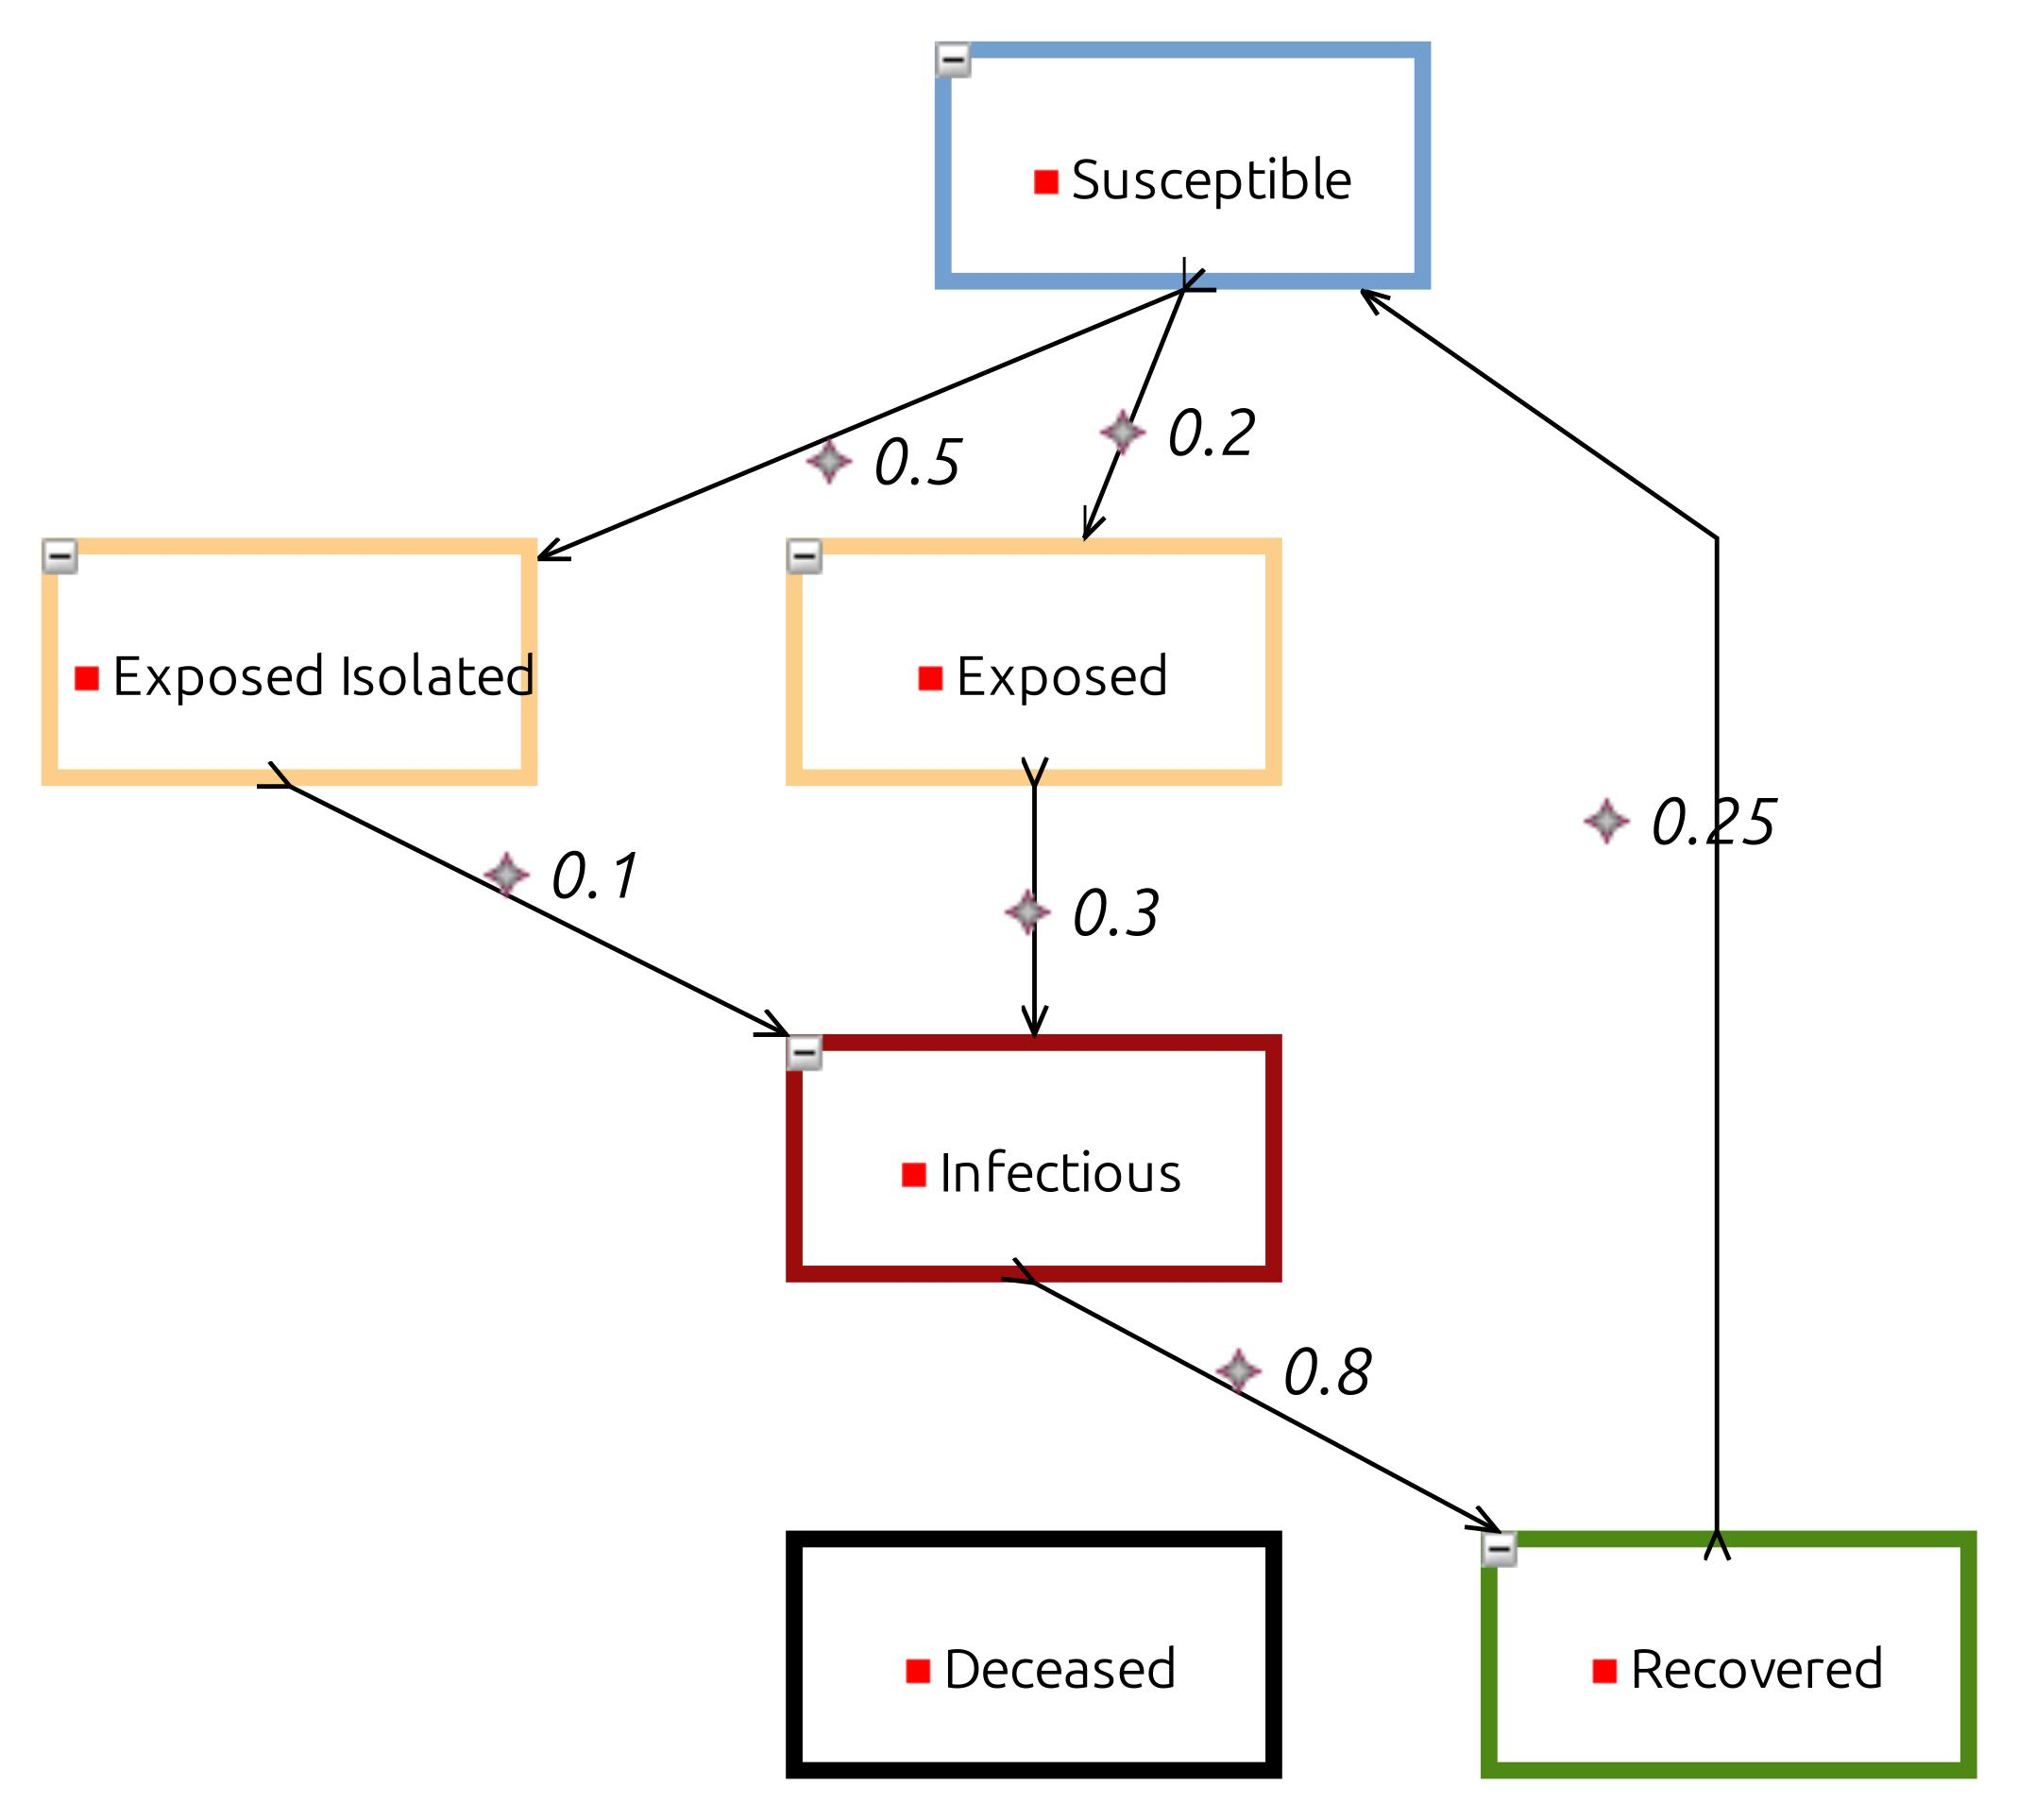
\includegraphics[width=0.5\textwidth]{Figures/fig9.jpg}
  \caption{The generated partially completed prototype model in EpiMDE containing Carol's selected features.}
  \label{fig:prototype_result_model}
\end{figure}

% \subsection{Discussion and Future Work}

